\documentclass[]{usiinfbachelorproject}
\usepackage{subfig}
\usepackage{caption}
\usepackage{subcaption}
\usepackage{float}
\usepackage{listings}
\captionsetup{labelfont={bf}}

\newcommand\subsubsection{\@startsection{subsubsection}{3}{\z@}%
                {-3.25ex\@plus -1ex \@minus -.2ex}%
                {1.5ex \@plus .2ex}%
                {\normalfont\normalsize\bfseries}}
\newcommand\paragraph{\@startsection{paragraph}{4}{\z@}%
                {3.25ex \@plus1ex \@minus.2ex}%
                {-1em}%
                {\normalfont\normalsize\bfseries}}
\author{Francesco Saverio Zuppichini}

\title{Design Interactive Display Applications for Active and Walk-by Contact Personalization}
\subtitle{The (optional) subtitle}
\versiondate{\today}
\begin{committee}
%With more than 1 advisor an error is raised...: only 1 advisor is allowed!
\advisor[Universit\`a della Svizzera Italiana, Switzerland]{Prof.}{Marc}{Langheinrich}
%You can comment out  these lines if you don't have any assistant
\assistant[Universit\`a della Svizzera Italiana, Switzerland]{}{Ivan}{Elhart}
%\assistant[Universit\`a della Svizzera Italiana, Switzerland]{}{AssistantName2}{AssistanSurname2}
\end{committee}


\abstract {
Nowadays displays are everywhere. They are mostly used to show information to huge amount of people by using a passive and unilateral channel. Our application, \emph{Tacita}, reshape that channel by creating a bilateral relationship between the user and such devices in order to provide in-walk personalised content.

Traditionally, personalization rely on user broadcasting their preference to a local display running an application without notify any other screen in the grid. With \emph{Tacita}, all elements of the architecture are aware of everything that may happen outside sharing a global state pushed into a reliable web socket proving a more convinient way to manage user's preferences.
}


\begin{document}
\maketitle

%%%%%%%%%%%%%%%%%%%%%%%%%
\section{Introduction}
\subsection{Motivation}

Big displays represent a widely used form of mass communication in almost all public places such as squares, subways and schools. They are used in a passive way by pushing un-targeted information, mostly advertisements, to the audience; enslaved by a unidirectional visible communication without any way to personalise the screen's content.

This lack of aimed informations brings to a uniqueness of the display's message, forced to be equal for everyone. Therefore, in the eyes of the device, is treated in the same way without making distinction. In the following pictures you can easily observe the abuse of this strategy by looking at two of the world's biggest squares that are invaded by static, brightly, unavoidable, content from the huge displays.
\begin{figure}[H]
  \centering
  \subfloat[]{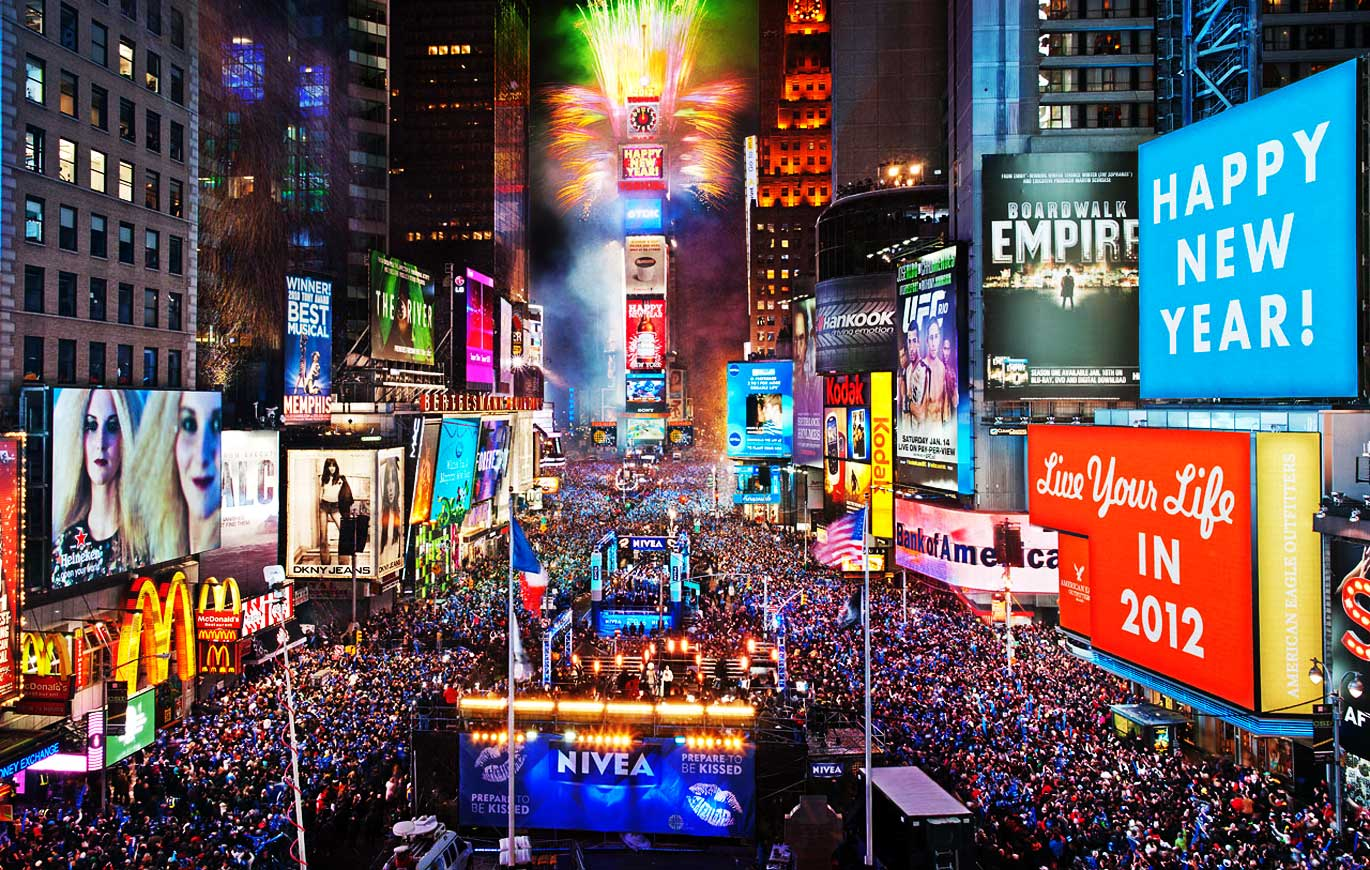
\includegraphics[width=0.43\textwidth]{./images/new_york_displays.jpg}}
  \hfill
  \subfloat[]{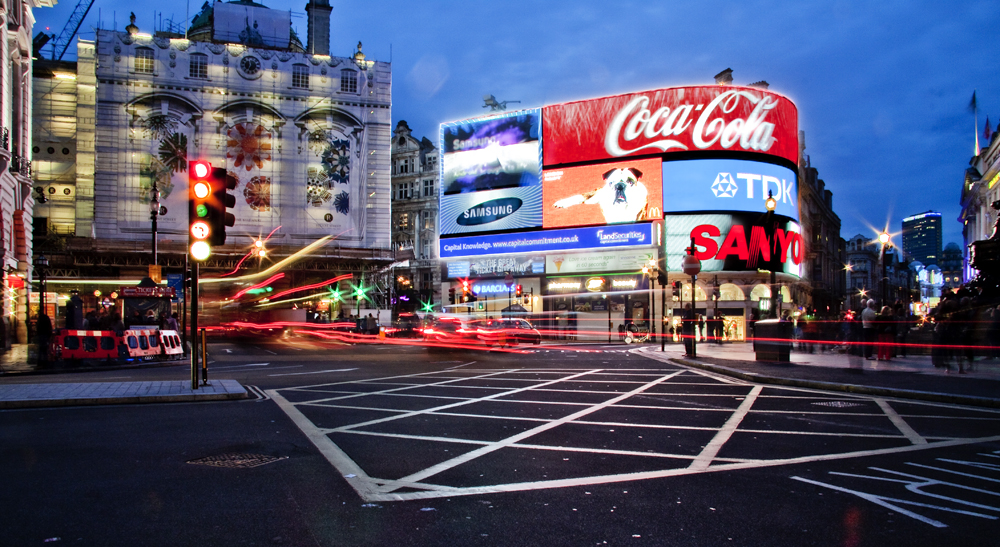
\includegraphics[width=0.5\textwidth]{./images/piccadilly_displays.jpg}}
\end{figure} 

Such devices make a big impact on a town's shape, they change it's look, colours and feel without adding anything useful. If we look in the pictures we can notice that the only content showed is advertisement. This choice is not directly related to the technology; in the following image, showing \emph{New York} in the early 60s, we can see the exactly same advertisement, even from the same companies, that is showed today. Therefore, even if the hardware has changed, it had not lead to an evolution of the context in which is used.
\begin{figure}[H]
  \centering
  \subfloat[]{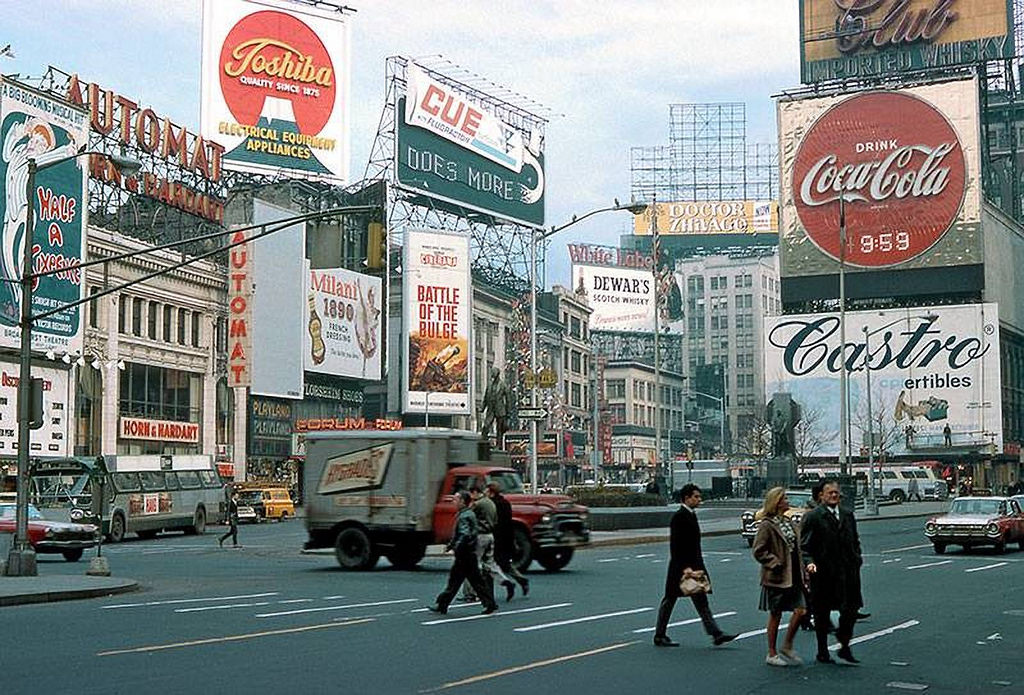
\includegraphics[width=0.5\textwidth]{./images/new_york_posters.jpg}}
\end{figure} 
The display's message is shared, or forced, to everyone; thus it seems logic thinking that everyone should share the screen too, but that is not the case.

A unified message cause a certainly reduction of the device's utility and purpose, making it, as we stated before, a full passive element. An other example of a badly use of displays may be the ones in the Milan \emph{Stazione Centrale}, showed in the following picture.
% add picture
\begin{figure}[H]
  \centering
  \subfloat[]{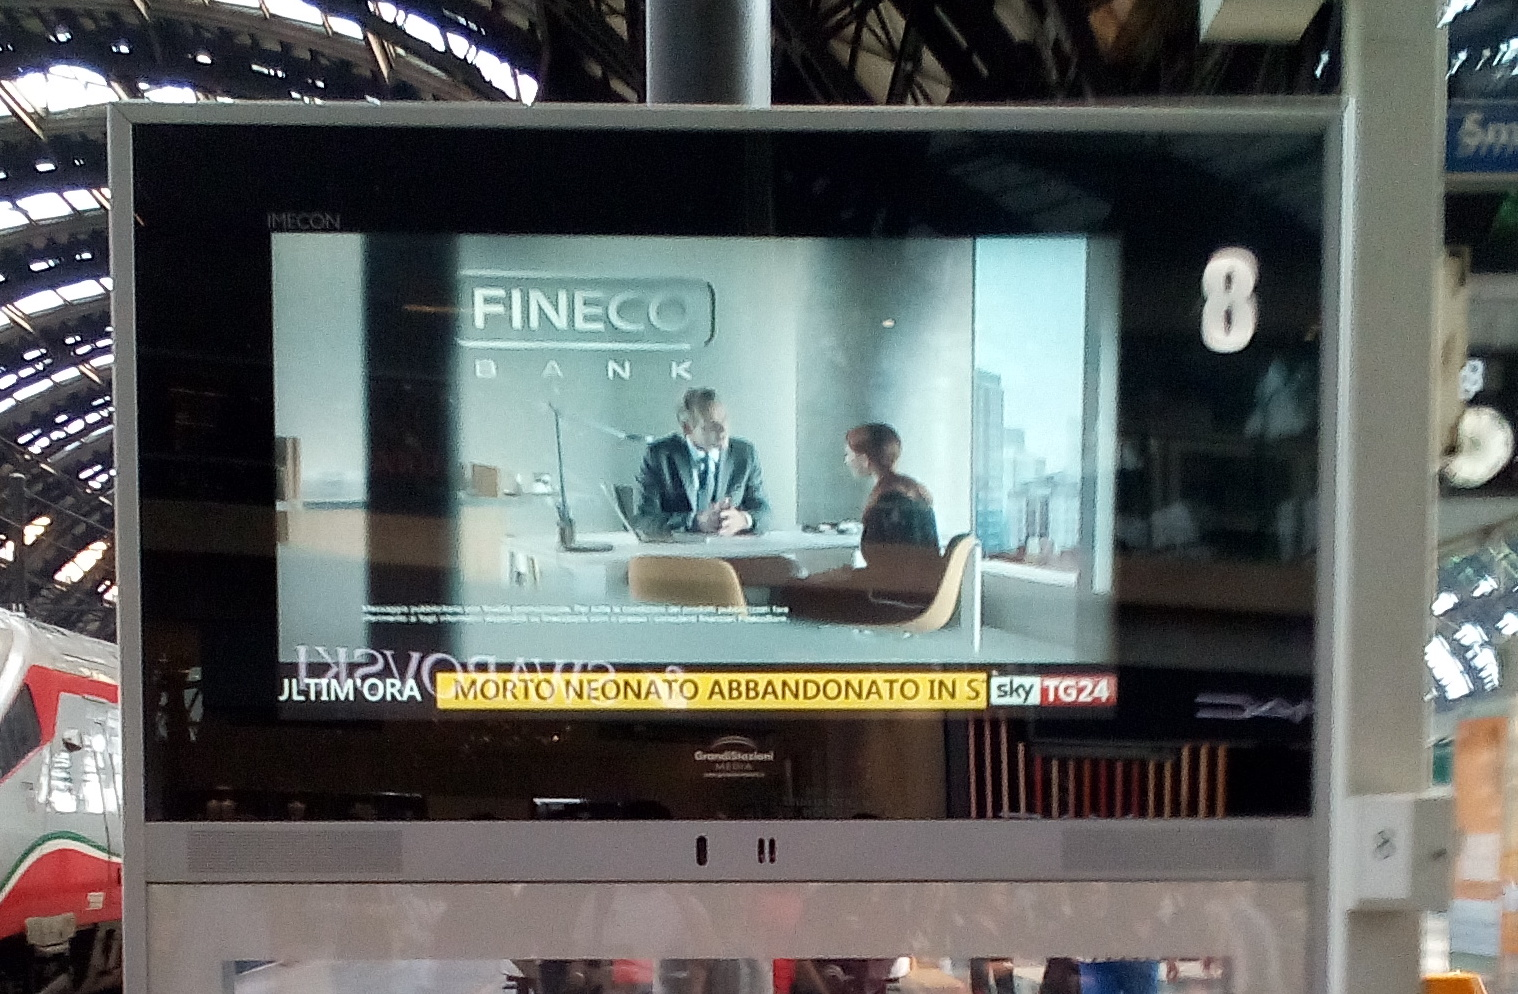
\includegraphics[width=0.5\textwidth]{./images/display_milano.jpg}}
\end{figure} 
They are used only to show publicity from the TV's channels loosing all the power that such devices embraces. Would be nice to just walk close to one of these and see our train schedules? Obviously yes.

An in-walk content personalisation is a logic step to made for using the full potential of such devices.
\subsection{Goal}

Our goal is to create a bi-lateral channel with the screen: the user must be able to quickly filter the information that he needs in just few seconds without being shelled by tons of useless brands and images. As it is deeply described in the next sections, in our architecture, the user is the active trigger that push and pull it's personal content directly into and from the display. This informations can be showed by just walking to the screen thanks to proximity sensors such as bluetooth beacons allowing a non blocking information flow where only the relevant content is target to the interested user at the right time.
\\
\\
The showed content must be pertinent and \emph{fast}, it must be easy for the user to enter the network becoming a part of it without loosing any time. For this reason we focus our attentions of the design part, aimed to provide a natural way of interaction between the system. Tons of studied shows the connection between poorly user interaction and high learning curve. Since we are addressing a endless mass of people, our application must be easy to start with and addressable. Therefore we decide to use smart phones as mainly platform
% ADD SOMETHING talk abou speed and user interaface with the smartphone
By doing that we completely transform a tool, such as a display, into a new one, a better one.
% say something of how software can change hardware an it is the main layer

\subsection{Results}
%As it will be deeply explained in the pages, we successfully create a fully functional architecture that allows to create a bidirectional communication channel making the display also an \emph{active} a that changes dynamically based on the users interactions. Our project uses a main application, called \emph{Tacita}, to provide the necessary instruments to create, manage and personalize preferences. A common interface is exposed from each Application using a Micro Services approach in order to make it easy to add new functionalities without interfere with the others elements.
%A touch display is used as main platform to show target content providing even more actions to the user that can just click and discover useful information.
We created a network that allows user to create, manage and see their preference by just walking nearby one of such devices. Moreover, they are also used in a old fashion way to show content on the fly by using the touch interface.
Each application is individually deployed by each provided without effecting in any way the system thanks to a micro services approach. They expose the same structure allowing a quick developing and integration in the network. The main entity that handles all the logic interactions between users, displays and beacons is \emph{Tacita}. It provides a solid web socket channel to push/pull notifications such as when somebody walk near a screen. It also stores all the components state providing a way to reach the applications from the mobile client to create personalized content.

A clean design is used as communication way to let users enter into the architecture without creating any account. The existing phone's account email is used to create an unique identifier entry into the database allowing a quick and safe access to the application. The smartphone is used to discovers displays thought bluetooth beacons connected to them. When one of those is reach, it starts pooling data from its application and display the user's preference using a colour base approach providing anonymity. 

\section{Architecture}
In this section we describe in detail the whole project design, bottom-up. Starting by a briefly description of how we structure all the parts.
\subsection{Introduction}
% INTRODUCTION
Design a full working system is never easy job. It has to logically mimic the answer to the problem we are trying to solve.

In our case, we are looking for a scalable system where the user, identifier as an active entry, pull and push his information to the display. It must not directly depends on the number of application, or \emph{services}, that our network exposes or on the number of display. Specifically the system has to work with $n$ display and $m$ application without any changing in the core. 
% GENERAL OVERVIEW
\\
\\
For such reasons we adopted a \emph{Micro Services} architecture where 

each element can be removed without effecting the global integrity. Services communicate using either synchronous protocols such as HTTP/REST; thus they can be developed and deployed independently. Each service has its own database in order to be decoupled from other services. Such architectures scale faster than a classic monolithic approach, for instance, a new application can be deployed from everywhere really fast by just using the same interface of the existing ones. Moreover, each application can be added from everywhere allowing developers to use their favourites technologies and hosting platform.
In our project we deployed all the services on the same server, but in a real world, as we said,  they are usually physically separated. Since all the applications provide a common interface for pull/push personalization content, we are going to call this set of services the \emph{Application Layer}.\\
\\
All the active logic of the network is handled by another Micro Service, called \emph{Tacita}, that links display, application and users. It's responsibility is to be the glue between the \emph{Application Layer} and all the other elements by storing users' informations, screen's state and available applications.
% TALK about the system that must be anynimous 

\subsection{Architecture Elements}
\subsubsection{General Overview}

We talked superficially of the elements of our Architecture: it is time to deeply describe them one per one. We start from the most important one: The User  
\subsubsection{User}

The User has a fully active role, he is the trigger of the whole system; without him, the network has not reason to exits. He uses his smartphone in order to access the front-end application exposed by the \emph{Appliction Layer} through the \emph{Tacita} platform.

By using it the User can selects his custom settings in order to quickly identify his information on the screens.
In our design, a favourite colour can be selected in order to filter fast the owned content and gaining anonymity, since nobody else can know who is linked to a specific colour. Also, colour base information can be identify really fast by just watching the screen.
This application will be deeply analized into the next sections, but, from a user point of view, it is the door to access the whole array of services.

We talked about the User as a \emph{trigger}, it means that, with his physical being, it \emph{triggers} actions; actions that are universally recognizable by our architecture. While walking near a screen, the architecture, thanks to bluetooth beacon that map them in the space, and, thanks to the smartphone application, can detect the movement show the personalized content into the screen at the right time. For the client, this is very convenient, since no other interaction is needed at all. One challenge we encountered was to make sure that the required content is showed in the correct time because, if the architecture is unreliable for the user then nobody will trust to use it.
 
\subsubsection{Display}

Display represent our \emph{tabula rasa} in which a wide array of applications can be showed. By default it can be identify as a \emph{passive} entry, but, combined to the User becomes the second \emph{active} element of our architecture. It makes possible to create a two way communication channel between by using a web socket and bluetooth beacon that is notifies the \emph{Tacita} application when a user walk next to a screen. Such information is used to push into the socket the user unique identifier. As soon as the display receives it, a request to the running application is made in order to get the preferences and showed them. Since we are using a common \emph{interface} in the Application layer, each of them expose the same structure to perform CRUD operations, the screen can create the same request structure without being bound to a specific application.

In our design we decide to only send the minimum amount of data that the is needed, delegating to the screen's software the work to fetch further informations making the socket channel faster and more flexible. The less the display needs, the better. Every time a user walk near display one, a notification is pushed of the following form is pushed into the socked allowing real time notification:
\begin{lstlisting}
{type:"USER_NEARBY",
payload: {id: "1" }
}
\end{lstlisting}
\\
As soon as it is received, the display, makes a request for asking for the user's preference:
\begin{lstlisting}
<TACITA_URL>/<APPLICATION_NAME>/api/preference/<USER_ID>
\end{lstlisting}
After success, it, obviously, displays them.
Since in each client used a Flux architecture, see SECTION NUMBER, the previous action based JSON will be globally recognize.

% add photo of the user display interaction
In our project, we used touch display with an Intel Nuc to drive them. Thanks to the touch interface, we can exposed an additional communication channel allowing user to quickly get content without being chained to the \emph{Tacita} application. For instance, everybody can to click somewhere in order to reveal a specific content, for example, a bus schedule.
  
\subsubsection{Tacita}
In the previous sections we have said that \emph{Tacita} is the glue of the architecture: it allows communication between users, display and application layer. In order to do so, we create a database's entry for each of these elements and we linked them with the correct relations. Since we are using MySQL we can take advantages of the relation structure that is imposed. A \one to one relation is create between the Display and the Application table, since, a single screen can run only one application at the moment. Also, when the the service is changed, the display automatically notify all the client connected to the web socket of the new state allowing each user to know in real time which application is running where.

Since \emph{Tacita} allows to enable and disable custom services, a many to many pivot is used to keep track of local user's applications state. If an application is turned off and a user is near to a display that runs that application, then no interaction between the two will happen. In our design, this check, is done on the client side giving to the display even more independent.
The physical device that make the in-walk communication possible is the bluetooth beacon produced by Estimote. Thanks to the custom android SDK provided by the manufactore, we can know exactly in which monitoring "region" somebody entered. On the server side, a one to one relation between Beacon and Display is created in order to quickly know, based on the beacon unique Id, which display is linked to. These devices must be putted really close to the machine we want identify in order to increase the location accuracy. Moreover, thanks to our API design, they can be changed at any time by just send the correct request to the server.

\begin{figure}[H]
  \centering
  \subfloat[Relations in Tacita Database]{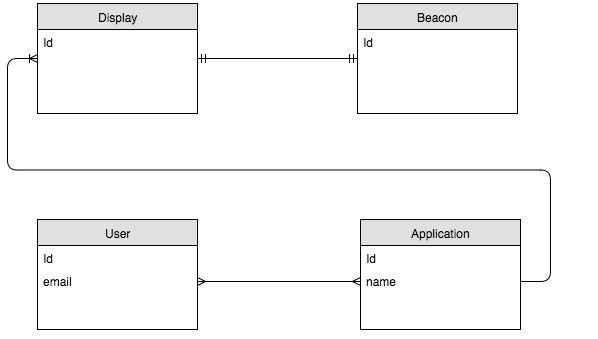
\includegraphics[width=0.5\textwidth]{./images/TacitaRelations.jpg}}
\end{figure} 




We also store the user information, such as email and favourite colour in another table. No login is required, the email is fetched from the mobile app when it boots and used as identifier. 

\subsubsection{Transport Micro Service}
The \emph{Transport} application allows users to navigate the nearby bus station and create preferences through the mobile interface. We decided to gather the data from the Opendata API that provides a set of well designed endpoint for fetching all kind of transportation information, in our case we used only the buses. However, due to the limit number of request we can made, fixed to three per second, and the necessity to have some custom endpoint, we cloned them.

We also have integrated Google Maps API into the screen's front-end; so, after fetching the exactly display's position thanks to web browser geo localization, we can show the estimate time to get to a specific station by walk. Imagine the benefit for a user to have know the minutes he needs to get to a nearby station, also, we can create a visible feedback before it is too late to reach them.

Using API and built-in browser geolocation make our system really scalable. Image you need to move the display to one location to another, with our system there is no need to update its state into the server since the information is fetched client side. So as soon as a display is moved, its position is updated as well with all the other functionalities related to it; therefore no external operation is needed.
One of our feats was that, cloning Opendata API, we loose all the benefits such as know if a bus is delayed; but in reality such information is always null. So, we have to assume that even them can not have access to such detailed information.
% say how ofter we clone them
% link to opendata
% put some pictures of the screen gui
For what the mobile application, as we talked before, it is made following the required interface. When it is loaded through \emph{Tacita}, the user can create, remove and update his preference. Each of these must have a station as mainly identifier, and an illimited number of buses.
% show some pictures of the preference flow
\subsubsection{Classes Micro Service}
The second implemented application is \emph{Upcoming Classes}, as the name says, it is used to provide the faculty student with useful information about classes such as the course schedule for the next days. Similarly to the Transport application, we had issues with the API, in our case, provided by the University itself.
A single API call to know all the schedules takes more than $1500ms$ as showed below;
% metti roba che le loro api fanno schifo
It gets worse if you try to get all the courses for a faculty:
\\
\\
\begin{tabular}{ l | c }
	Request & Time \\
	\hline
	http://search.usi.ch/api/courses/35255488/schedules & 1952ms \\
	http://search.usi.ch/api/faculties/1/courses & 9294ms\\
\end{tabular}
\\
\\
\\
% stessa di sopra
Therefore they cannot be properly used in a real application. Even if, from the client, we always cache the request, we cannot avoid to wait for the first time. The reason why they are so slow is the response size. Their response is heavy due to a poorly model population; for each course that is sent back, tons of unused field are provided. Also, by inspecting a response for a class schedules, we can notice the same huge course object appears, unnecessary, for each schedule object.
Therefore, again, we needed to clone all the API in order to just sent the right amount of information, by doing that, the previous schedule request now needs just $18$ms.
\\
\\
\begin{tabular}{ l | c }
	Request & Time \\
	\hline
	 http://tacita/classes/api/course/246/schedules & 18ms \\
	 http://tacita/classes/api/faculty/1/courses & 1000ms\\
\end{tabular}
\\
\\
\\
The display's front end application is divided into two main part easily identificable, the calendar and the query engine next to it. The calendar is create using \emph{fullcalendar} jQuery library that does all the dirty work of render and setting up all the events into the corrects slots. 
The courses can be selected thanks to the query engine on the right part of the screen. As soon as the user clicks on the button representing the faculty, it is guided in order to create a valid query using a step by step approach; even if it may be not the faster way, it is the safest since no wrong request can be generated. The procedure is shows in the following storyboard:
% aggiungi storyboard classi

As we did for the Transport Application, we also created a smart phone interface in order to create, remove and edit preferences. Since the interface is always the same we decided to also decide to keep the same design for consistency reason.
% show transport app similar to this one
\subsection{Architecture Interactions}
In the previous part we define in detail each element of our architecture without giving a global overview of how each parts collaborate with the all system. In this section we are going to analize all the interaction, especiatally between user and display, in detail showing each message that the entities exchange, explaing our design decision and analyzing the interactions.

From a User point of view, the first actions that can happen is walking into a display. As soon as the smartphone deteachs the beacons, they can talk to each other by exchanging information. The first message collected is the beacon id. After that, a request to \emph{Tacita} is made in order to know which display is associated with that beacon. If there is one, a message containing user's id and display's is pushed into the socket only if the screen application is enabled. As soon as the display receive the message, it checks if it has the same id; if so a request to out back-end services is made in order to get the user's preference. Finally, the user's content is showed into the screen.

The display does some additional actions. When he receives the preferences, it uses a in memory cache to avoid processing the same information two or more times. Also, a life duration is set for each of them in order to remove them if no exist event is detected.

Moreover, when a screen is deployed, it need a unique id to become officially part of the system. Such id is create thought a POST call to \emph{Tacita} and it is passed to the display by adding it in the end of the url that is processed by the front-end software.
Then, the newly created screen, can finally get the application by the correct micro service and display it.



\begin{figure}[H]
  \centering
  \subfloat[User interactions]{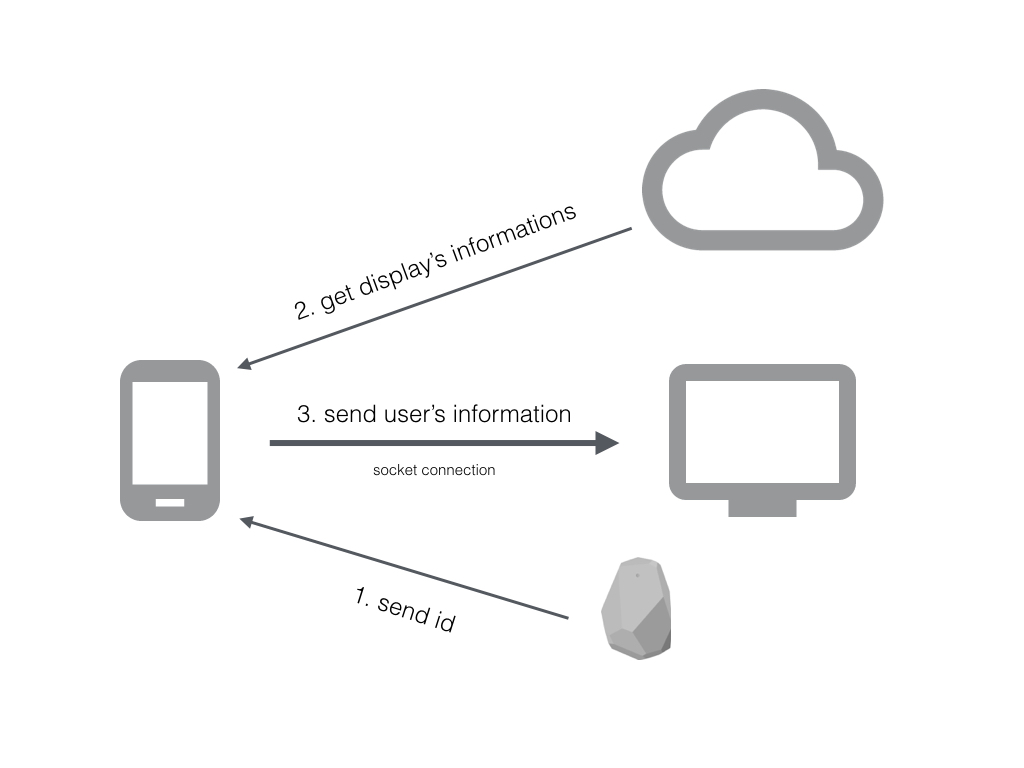
\includegraphics[width=0.5\textwidth]{./images/user_interactions.jpeg}}
    \subfloat[Display interactions]{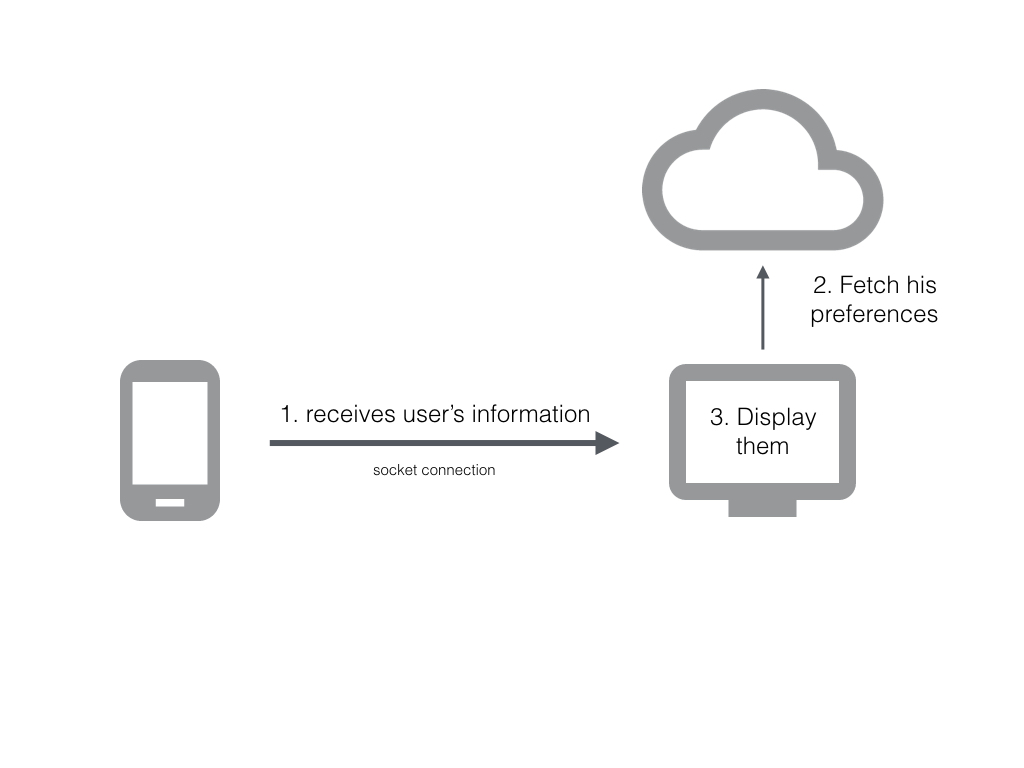
\includegraphics[width=0.5\textwidth]{./images/display_interactions.jpeg}}

\end{figure} 
\subsection{Architecture Technologies}
In this section we talk about the technologies that we used for the back-end and the front-end. For this project, we choose the latest technologies and programming languages in order to provide a service that will last without being obsolete in a long term.
\subsubsection{Back-End}
We firstly started to develop the first application using Django, a python web framework, but, even if its widely used among back-end developers, we encored problems with web socket that were not supported "out of the box".
So, we decide to completely switch both language and framework by choosing Swift 3 and Vapor.

Swift is a "powerful and intuitive" open source programming language developed by Apple in 2015 for booth MacOs X and Linux. It is a Protocol Oriented Programming Languages, quoting from Apple:
\\
\\
\emph{A protocol defines a blueprint of methods, properties .. The protocol can then be adopted by a class, structure, or enumeration - Apple}
\\
\\
Unlike classes, the fundamental of POP, Protocol Oriented Programming, programming is Value Type encouraging flat and not nested code. This benefit is reflected into its performance and flexibility.
The syntax is concise yet expressive, it uses labels and spaces to improve the code readability making possible to write complete sentences only with code. Apple wanted to create a product that was at the same time, feast and beauty.

After selecting a programming language, we need a framework to create our applications. We choose Vapor for the job; a powerful, beautifull and easy to use MVC framework to build web servers. In our project it powers all micro service including Tacita.
Vapor is easy to start with thanks to the clear APIs that, not also speed up the developer work, makes the code more maintainable and more understandable. One of his strength point is the performance inherited from Swift. You can see in the following table a benchmark in which Vapor outstands also the most blasonated framework such as Spring.
\begin{figure}[H]
  \centering
  \subfloat[Plaintext request/second]{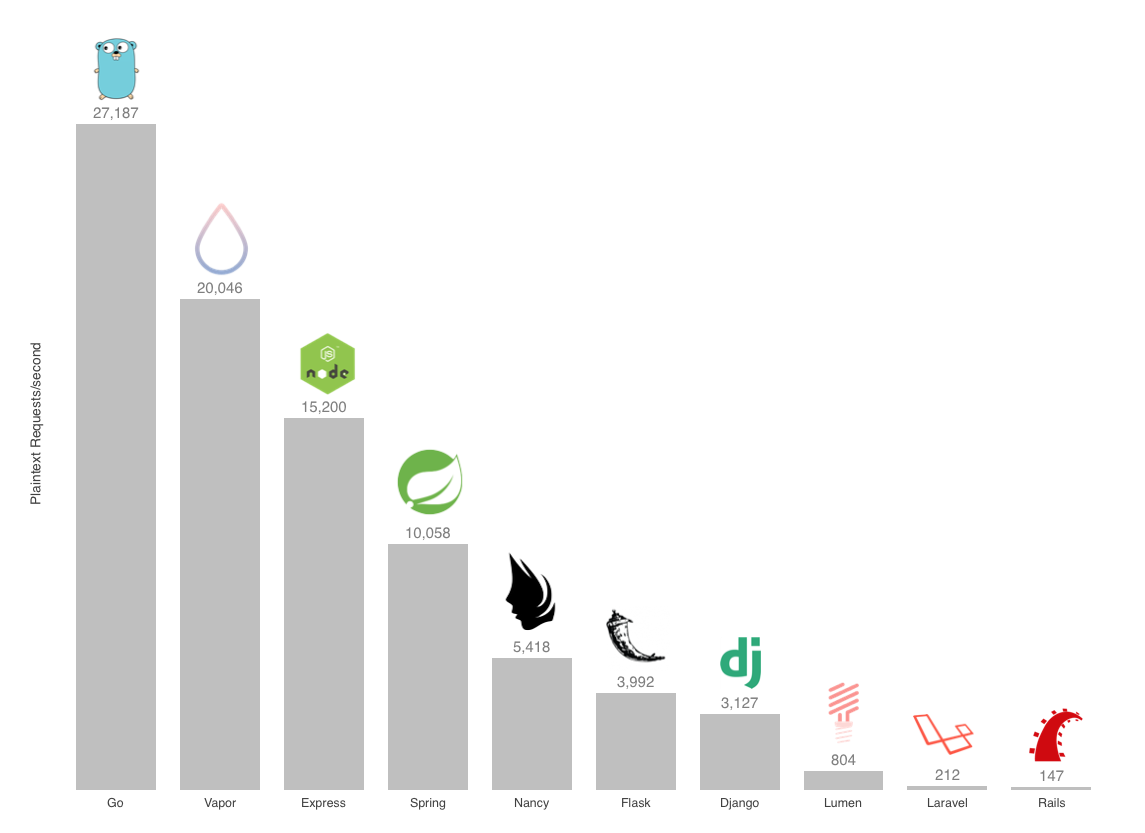
\includegraphics[width=0.5\textwidth]{./images/vapor_1_benchmark.png}}
\end{figure} 
% agginugu benchmark
\subsubsection{Front-end}
In order to archieve the best results in term of scalability and performance we choose Vue.js as main front-end framework. Vue.js is a library for building interactive web interfaces, it uses web components to provide a convenient way to organize an application by decoupled its element into blocks.
A web component is similar to a Object Oriented programming classes, it encapsulate all the logic behind a certain functionality of the application. In Vue, a component, in formed by three parts: template, script and style.

The template allows the developer to write html and include variables, conditions and loops. Also, thanks to build in loaders, is it possible to easily use any pre-processing html library such as Pug.
The second part is the core of each components, the script. As the name may suggest, it is the code part. Each component expose a javascript object allowing Vue to grab it and render it in the proper way.
The last tag is were is possible to style a component using CSS, as before, it is tremendously easy to use Less, Sass and other css-processors.
One of the main advantages of Vue over other front-end framework is \emph{reactivity}. Reactive programming is an synchronous programming paradigm concerned with data streams and the propagation of change. It uses Observers in order to trigger events every time a change of state is detected; therefore Vue can automatically call a render only in the part that was actually mutated minimizing the DOM access and increasing speed.
A deeply comparison with other frameworks can be fount at: https://vuejs.org/v2/guide/comparison.html. The following graph shows its performance against Angular and React, the other two most used framework developed by Google and Facebook respectively. We used Vue 2.0.
\begin{figure}[H]
  \centering
  \subfloat[Vue.js vs other popular libraries]{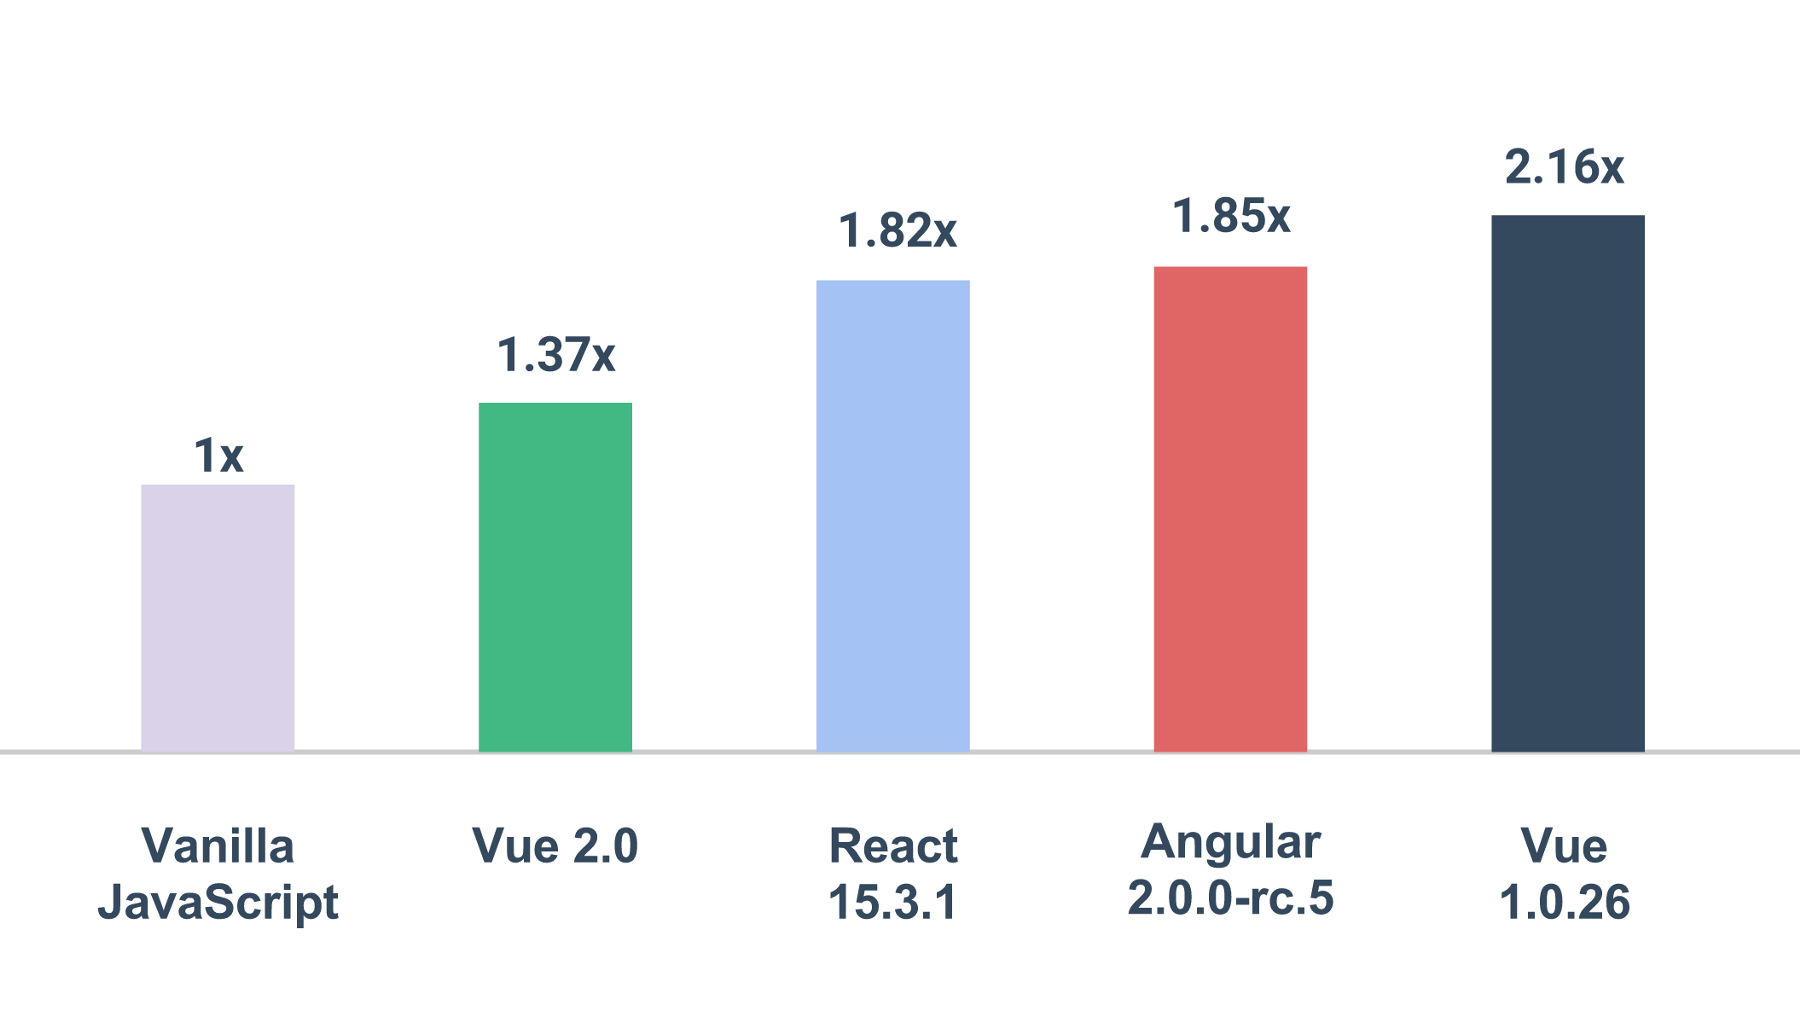
\includegraphics[width=0.5\textwidth]{./images/vue2_benchmark.png}}
\end{figure} 
As we said, each component represent a feature, a part of the web application; it may happen that one of them need to communicate with another, maybe after a change of state or a user event. In order manage the data flow we used the Flux pattern. The mainly idea behind this pattern is that the state can be mutated thought actions that are reduced into the stores. It is composed by four parts: Dispatcher, Store, Actions and View.

The dispatcher is a singleton that receives them and dispatches to every stores that have registered with it; its important to highlight that every store receives every action.

The Store is only source of truth in the applications; it holds its state and manage the logic behind it. The data must only be mutated by responding to and action by emitting a "change" event.

Actions are the internal API of each application, they define all the possible interaction that may happen. They are plain javascript object composed by a type field and some data.

Views displays store's data; in our application, a single view is a Vue component.

Even if there already exist a fantastic Flux library, Vuex, for Vue created by its author, we decide to create a new one from scratch. Our library, called Flue, aims to provide a better object oriented approach than the existing one. You can find examples and documentation at our Github repository: https://github.com/FrancescoSaverioZuppichini/Flue.

\begin{figure}[H]
  \centering
  \subfloat[Flux data flow]{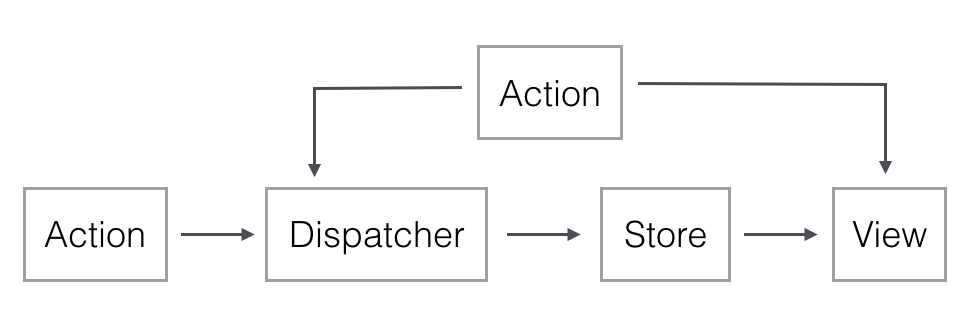
\includegraphics[width=0.5\textwidth]{./images/flux_data_flow.png}}
\end{figure} 
\subsection{Architecture Scalability}
Scalability is the ability of a system to grow larger with minimum changes. In the previous sections we often talk about how some design choices lead to an improvement in term of scalability. In our specific case, our system can change very quickly at any moment: just image if the provided buy new displays or new applications are available.

In order to make it possible to deploy independently from the network a new application, we abstract the its concept creating a layer of services that can be expanded very easily. The developers can create a new applications by just creating a web server being conform to our generic interface and expose his url.

Another possibile problem that can may appear is when a display is moved away. We explained before how each screen, when its connected, fetch its position and use it in order to communicate with Google Maps API to show real direction indications. If such problem appears, very easily, the provider just need to refresh the screen and the front-end software will automatically update itself.

Also displays can be removed or added by simply using \emph{Tacita} REST API. Imagine a screen brokes, then the associated beacon can be moved to another screen or the display may be replaced. The last case is the easiest, since we can just turn on the screen and use the last display's id, if no new devices is avaliable then the beacons can be quickly be linked to the a new screen.

\section{Design}
In our project design plays a key role. Since our applications can be used to anybody, a clear and effective interface is mandatory to ensure a global usability. Moreover, when dealing with big display, we have to provide a no blocking content flow meaning that an interaction should not prevent, or block, another. Also, all state changing must be displayed using design techniques, such as well targeted animation, in order to make the user understanding what is happening around him.

We decide to follow a \emph{content first} strategy by making the content clear and visible using a minimalistic approach; no unused element is present in any application. We used \emph{cards} as only way to organize information. In design, a card is a sheet of material that serves as an entry point to more detailed information proving a convenient way to display content composed of different elements.
% qualche foto di card
You can see notice how they are used in the Transport application as only data flow container.
% screen display Application

\subsubsection{Display}
The main challenge was to design for a big touch interface. We started by keeping in mind that every information must be quickly receable and accesible; the user must understand in a fraction of second what he needs. By keeping that constrains in mind.
Our design process starts with wireframes; representin the skeletron of the application exposing its main functionalities. They are terribly useful to get a first general look of what the application is going to be. For what It concern the Transport service, we begin by discard every not necessary element following, as we said, a minimilistic approach. In the following picture you can see the first wireframe's muck up and the final product
\begin{figure}[H]
  \centering
  \subfloat[wireframe]{\includegraphics[width=0.43\textwidth]{./images/transport_wireframe.png}}
  \hfill
  \subfloat[final product]{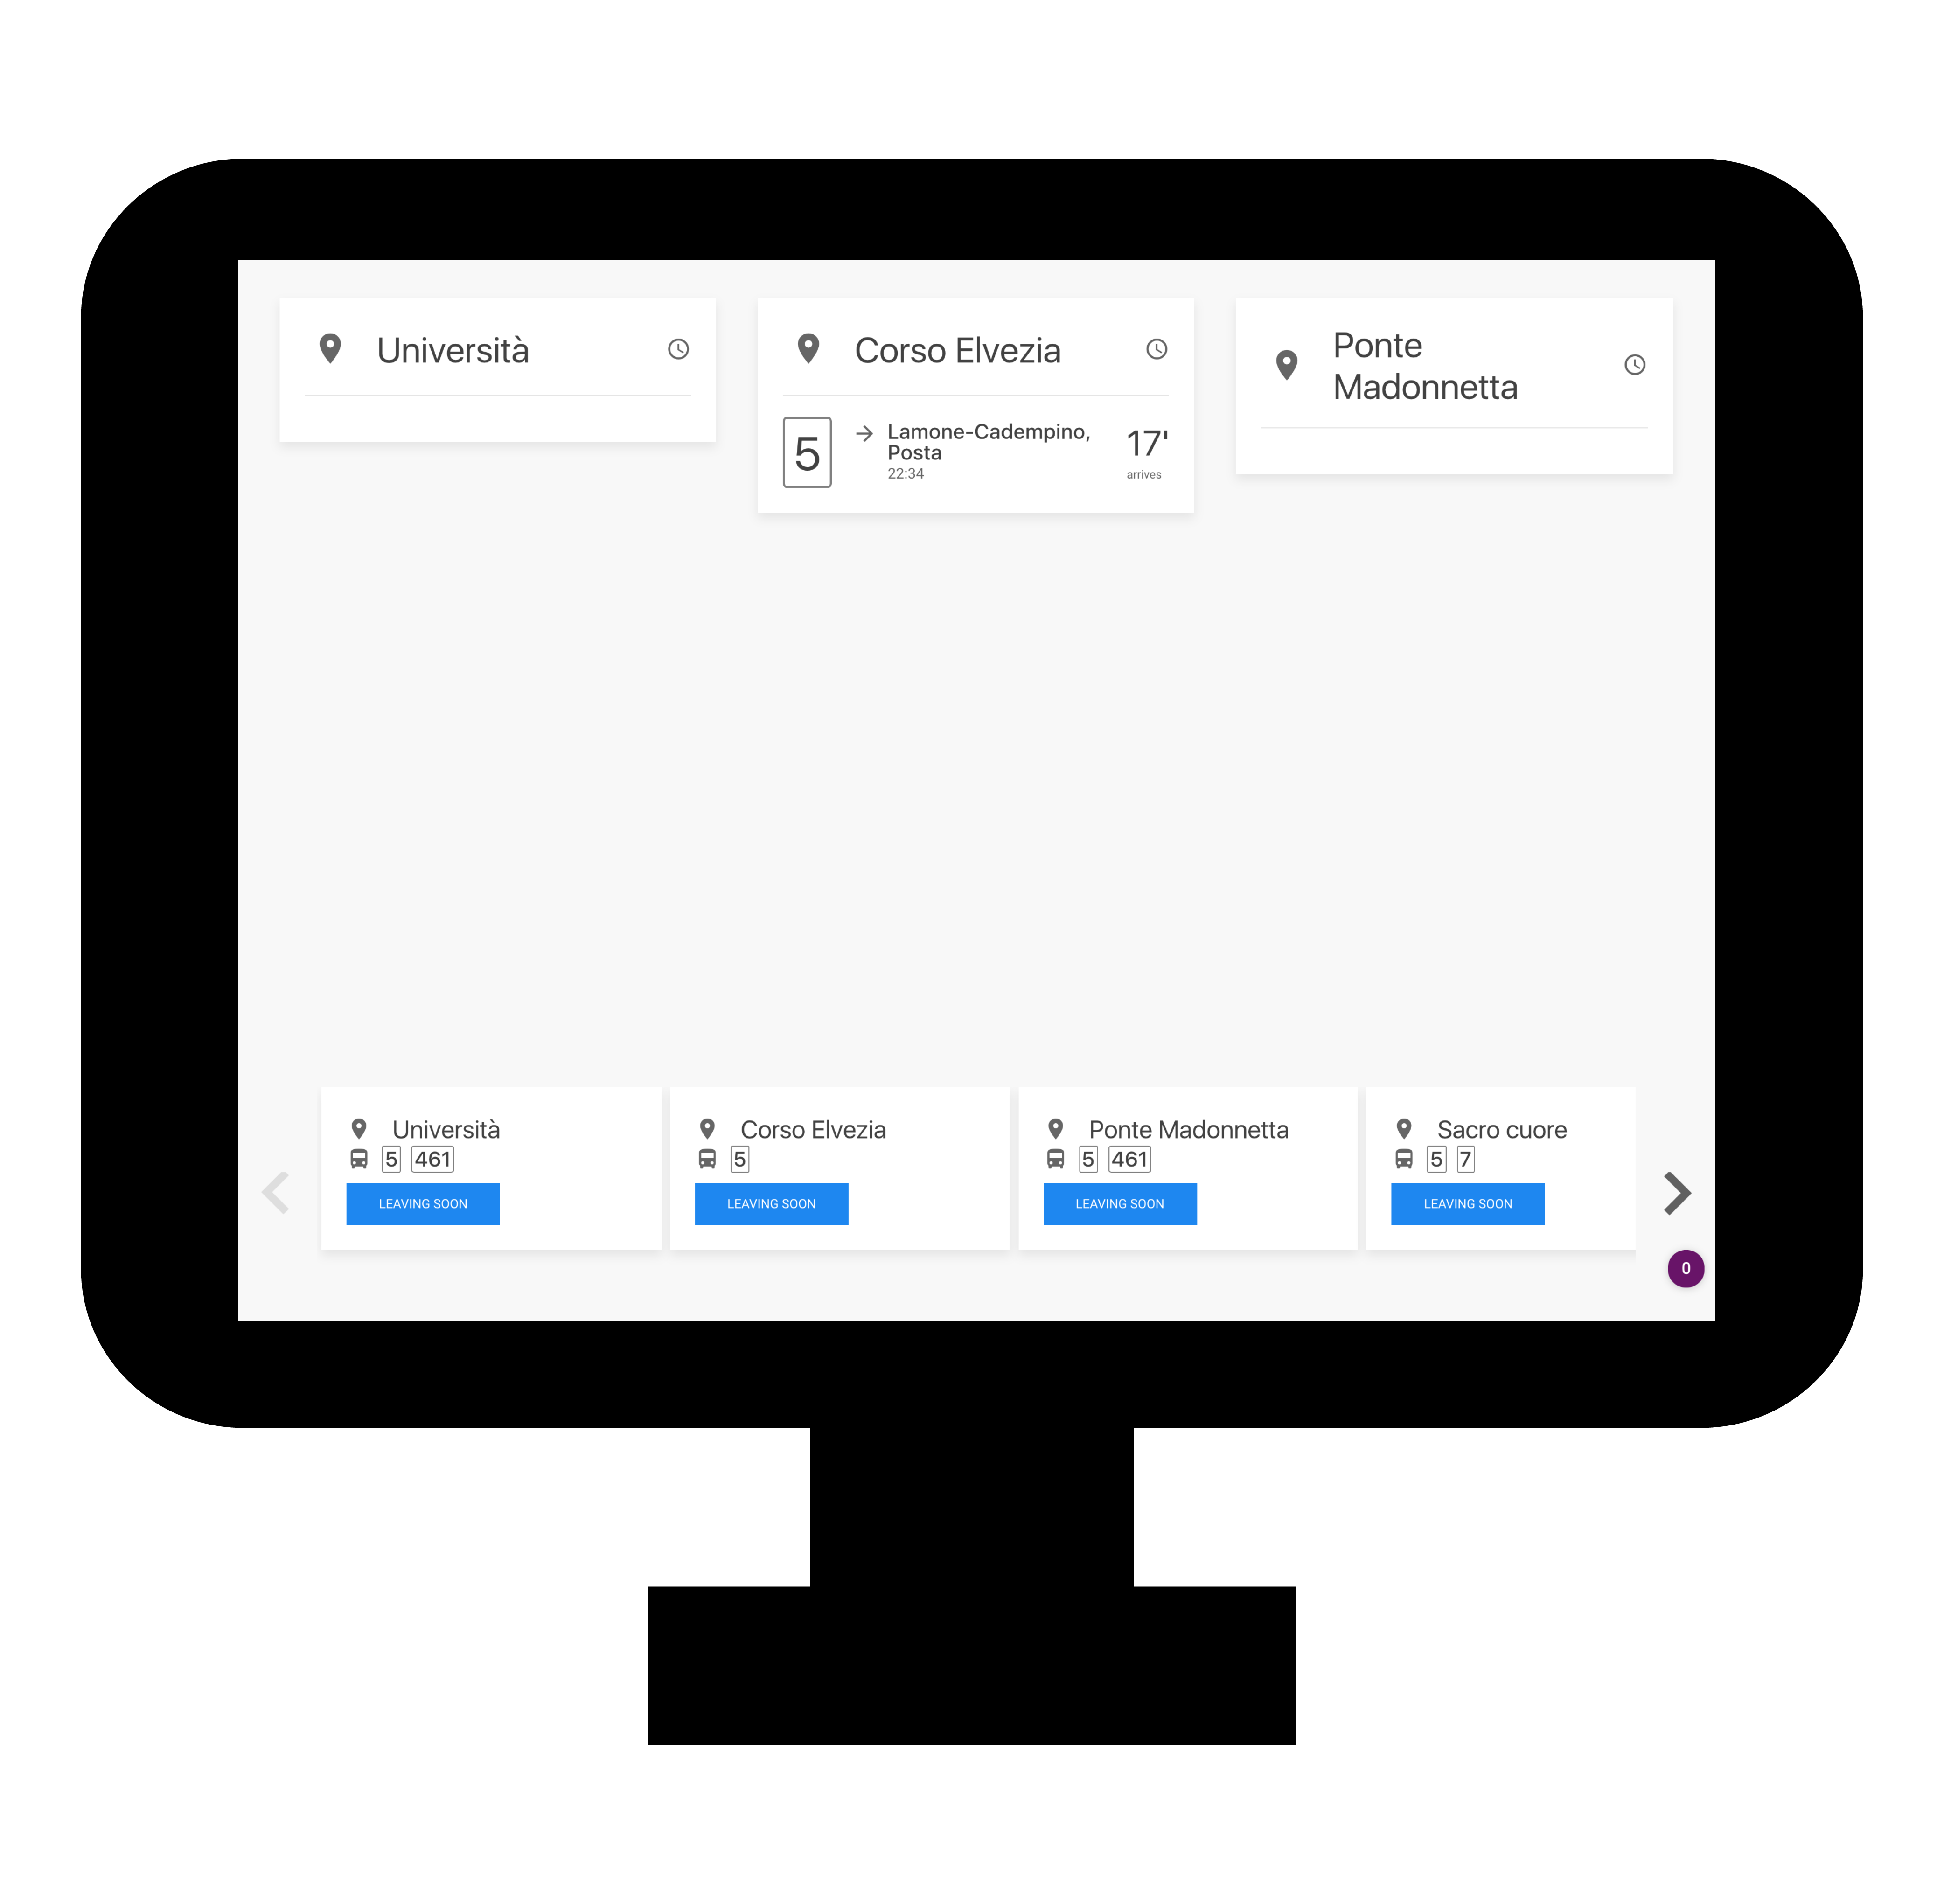
\includegraphics[width=0.53\textwidth]{./images/transport_application}}
\end{figure} 
If you look at the left image you can notice that all the functionalities are intuitively recognizable. As we said, our design, must be carefully studied for big display; we focus on the interactive part.
At the bottom of the application there is a carousel used to change station on the fly. All buttons are big enough to be easily be used from everyone without any problems.
Moreover, we used animation to increase the user experience; when a station is selected is pushed on the right part using a slide in animation making more visible. Also, a open station shakes when a user try to open it again giving a strong visible feedback of where it is on the display. 

In the Class application we used the same approach, we started by sketching the wireframes and defining the main functionalities. In this specific case, we need two components: a Calendar and a query engine to search courses. 
\begin{figure}[H]
  \centering
  \subfloat[wireframe]{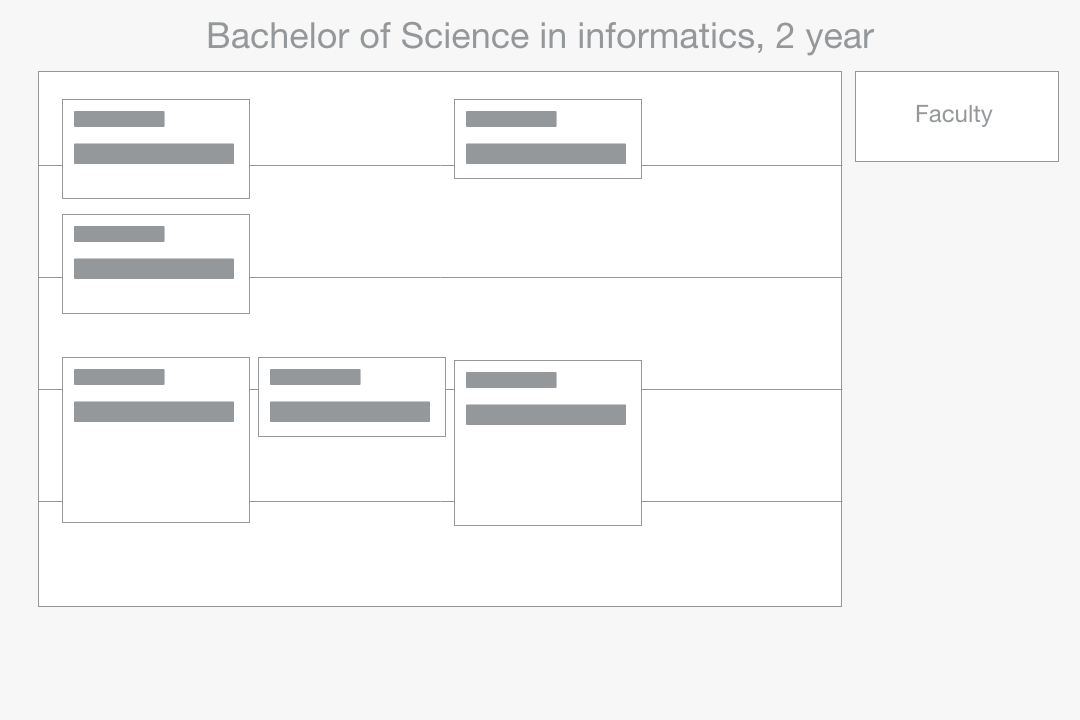
\includegraphics[width=0.43\textwidth]{./images/classes_wireframe.png}}
  \hfill
  \subfloat[final product]{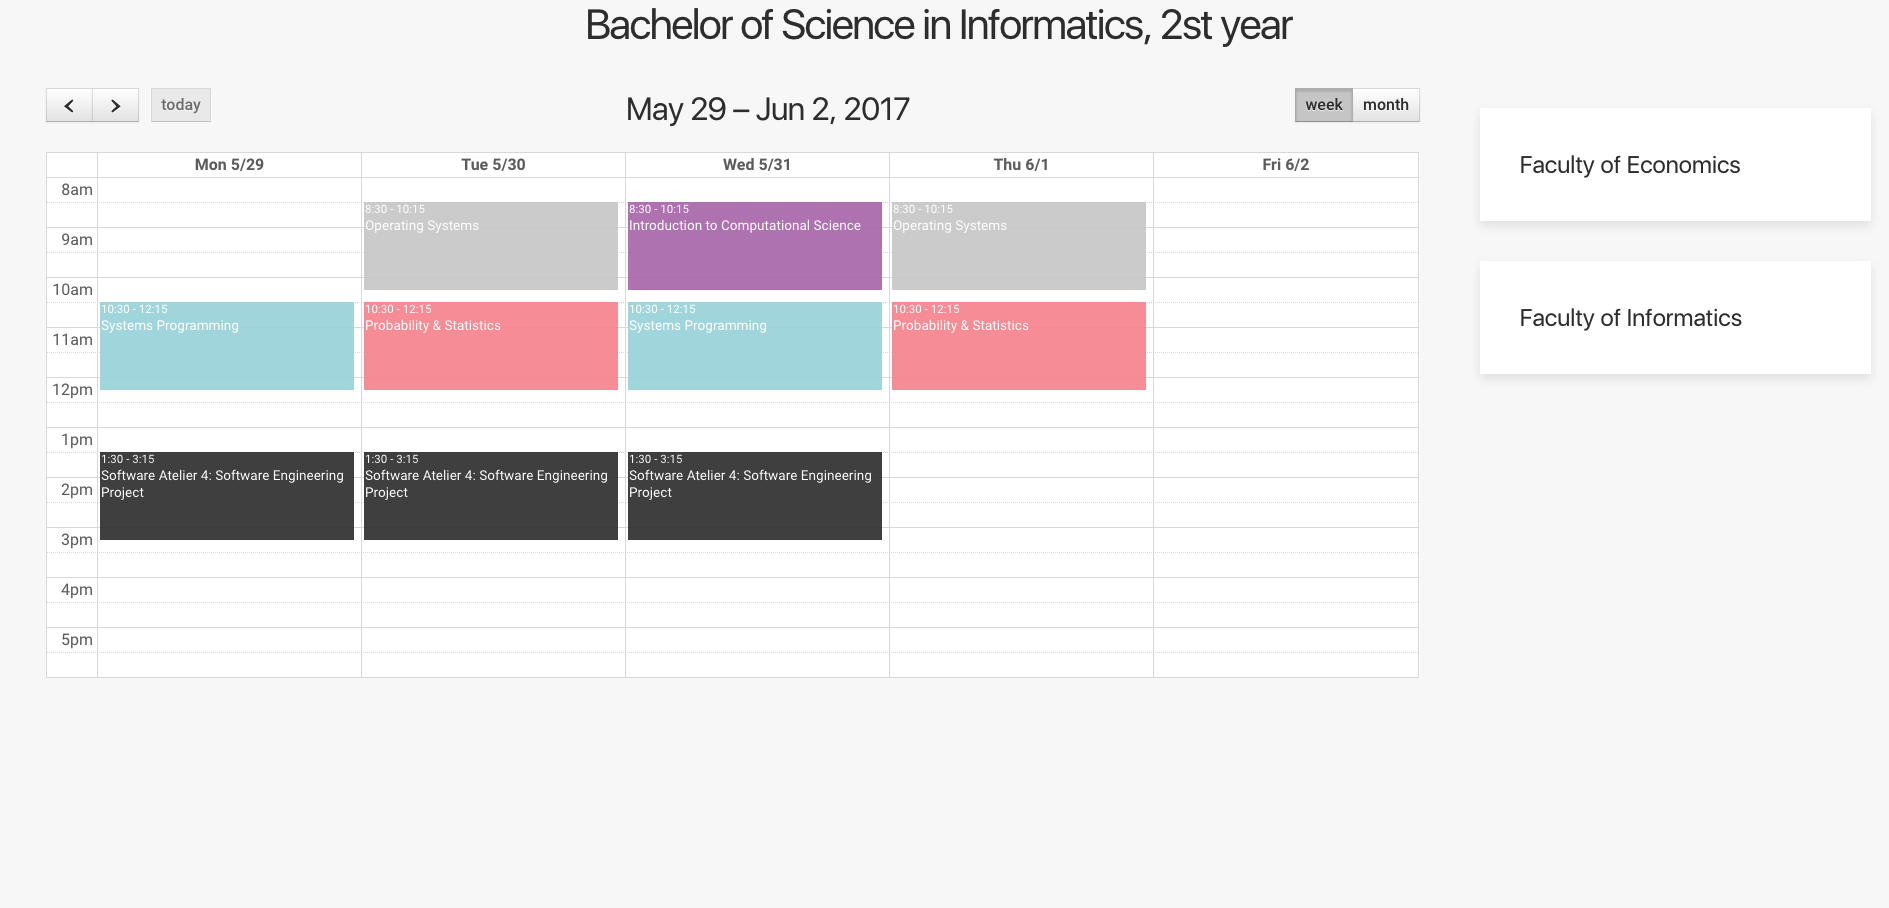
\includegraphics[width=0.53\textwidth]{./images/classes_application}}
\end{figure}
\subsubsection{Smartphone}
As we have explained before, we develop an smartphone application called \emph{Tacita} in order to organize the user interaction with the display. We design it from sketch to be accessible for everyone from everywhere. 
Logically, in main page of the application is possible to see and enable all the existing application exposed by the \emph{Application layer}. Since we wanted to provide a more comfortable user experience we added skeletron loader instead of a classic spinner; therefore, in case of slow internet, is possible to 'guess' the content of a page. The following pictures show the process.
\begin{figure}[H]
  \centering
  \subfloat[Loading]{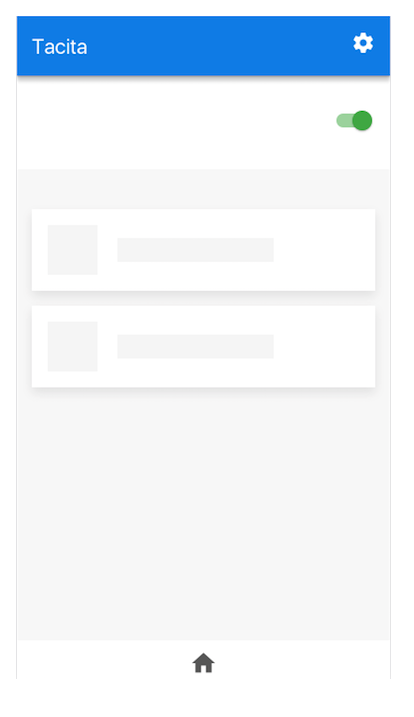
\includegraphics[width=0.25\textwidth]{./images/tacita_skeletron}}
  \
  \
  \
  \subfloat[Finish]{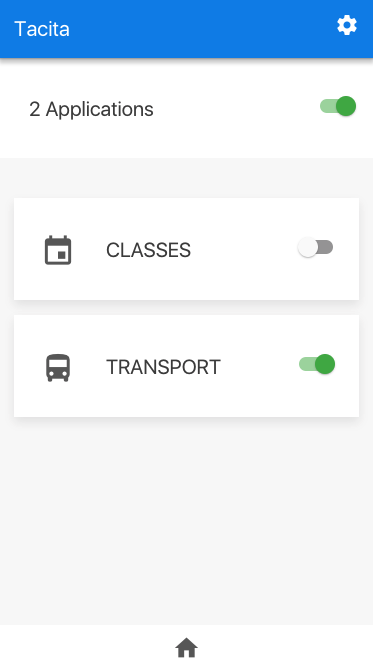
\includegraphics[width=0.25\textwidth]{./images/tacita_main}}
\end{figure}
As you may notice, is it easy to understand how the content
When a User walk nearby a screen a float button pops up making the displays page avaliable, and, since we are using socket connection, if the display changes the running application, the client will be notified

\begin{figure}[H]
  \centering
  \subfloat[Beacon found]{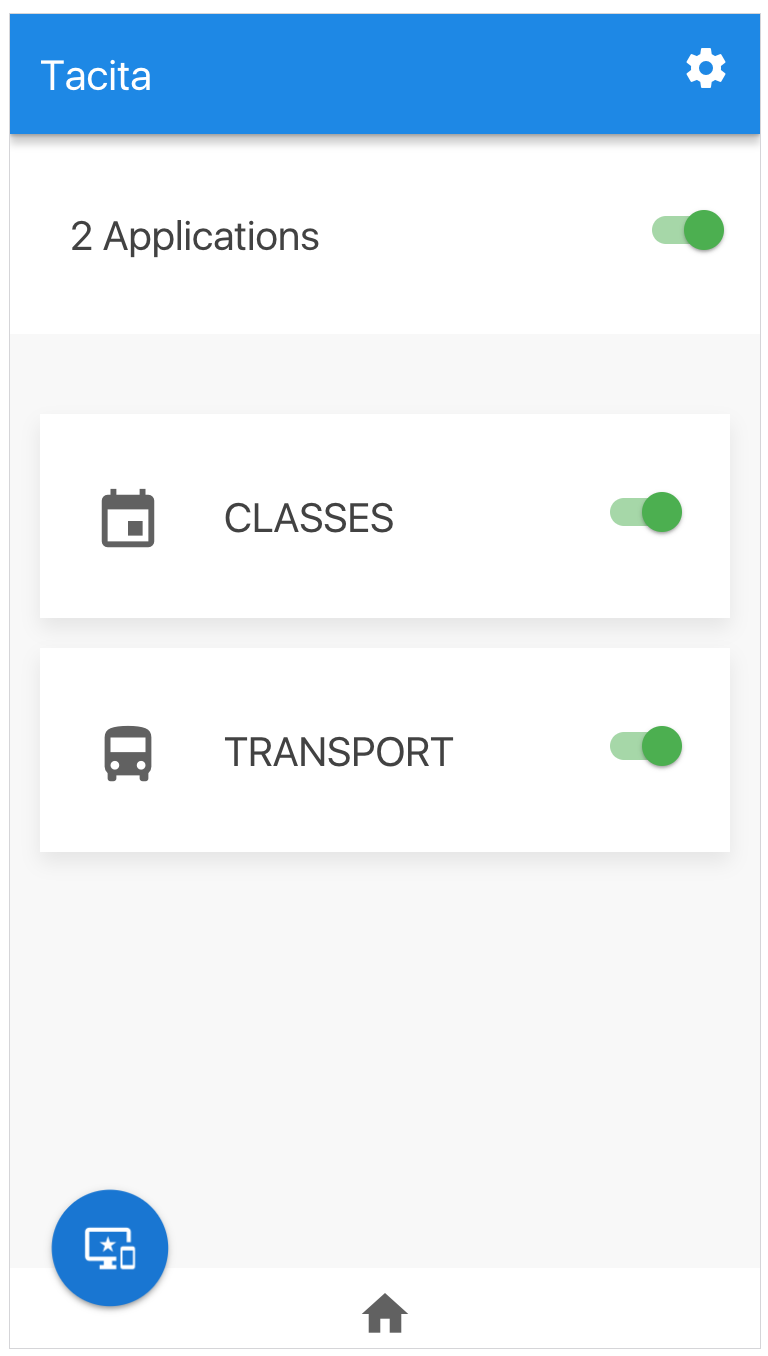
\includegraphics[width=0.25\textwidth]{./images/tacita_display_found}}
   \
  \
  \
  \subfloat[Display found]{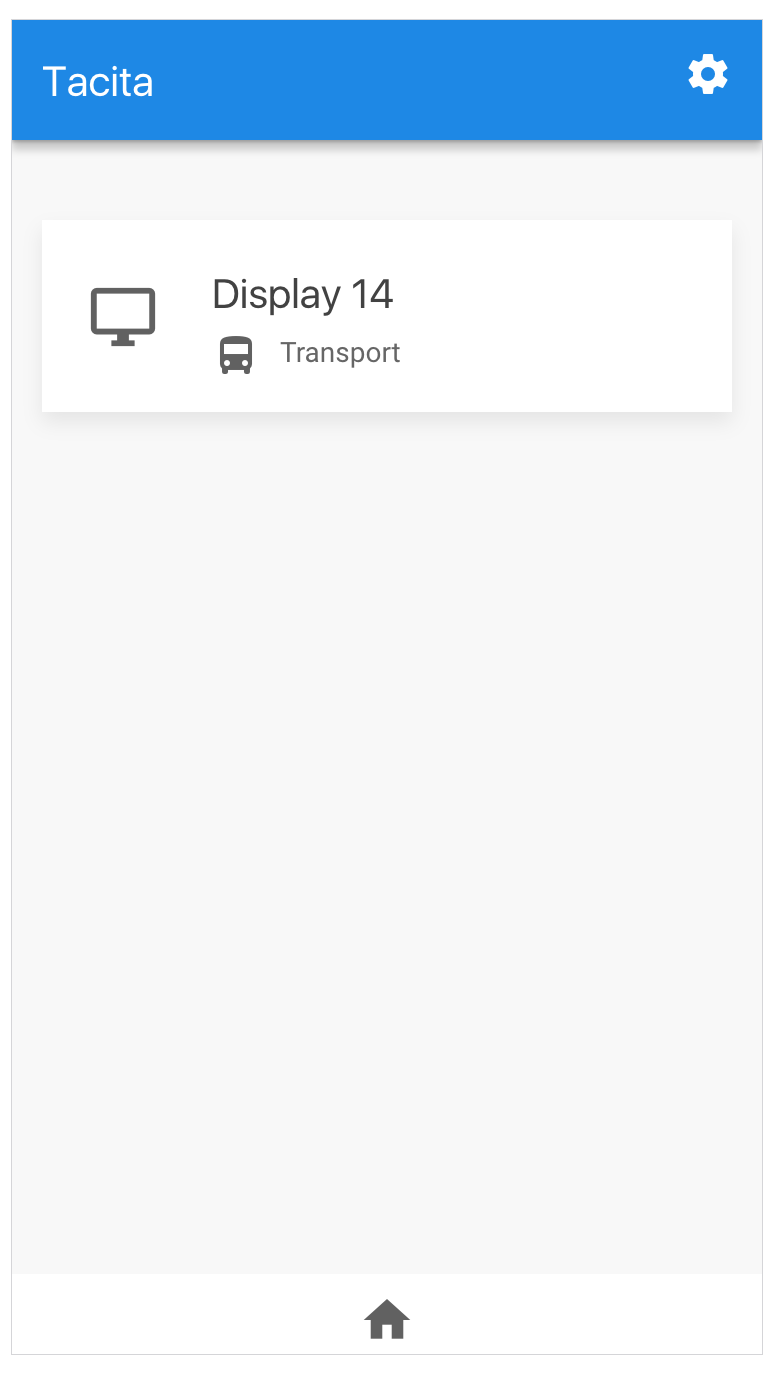
\includegraphics[width=0.25\textwidth]{./images/tacita_display_view}}
\end{figure}
We also provide a convenient way to select a custom personalisation. As we said before, we choose a colour based approach in order to highlight the visibility of a own content.

\begin{figure}[H]
  \centering
  \subfloat[Select a colour]{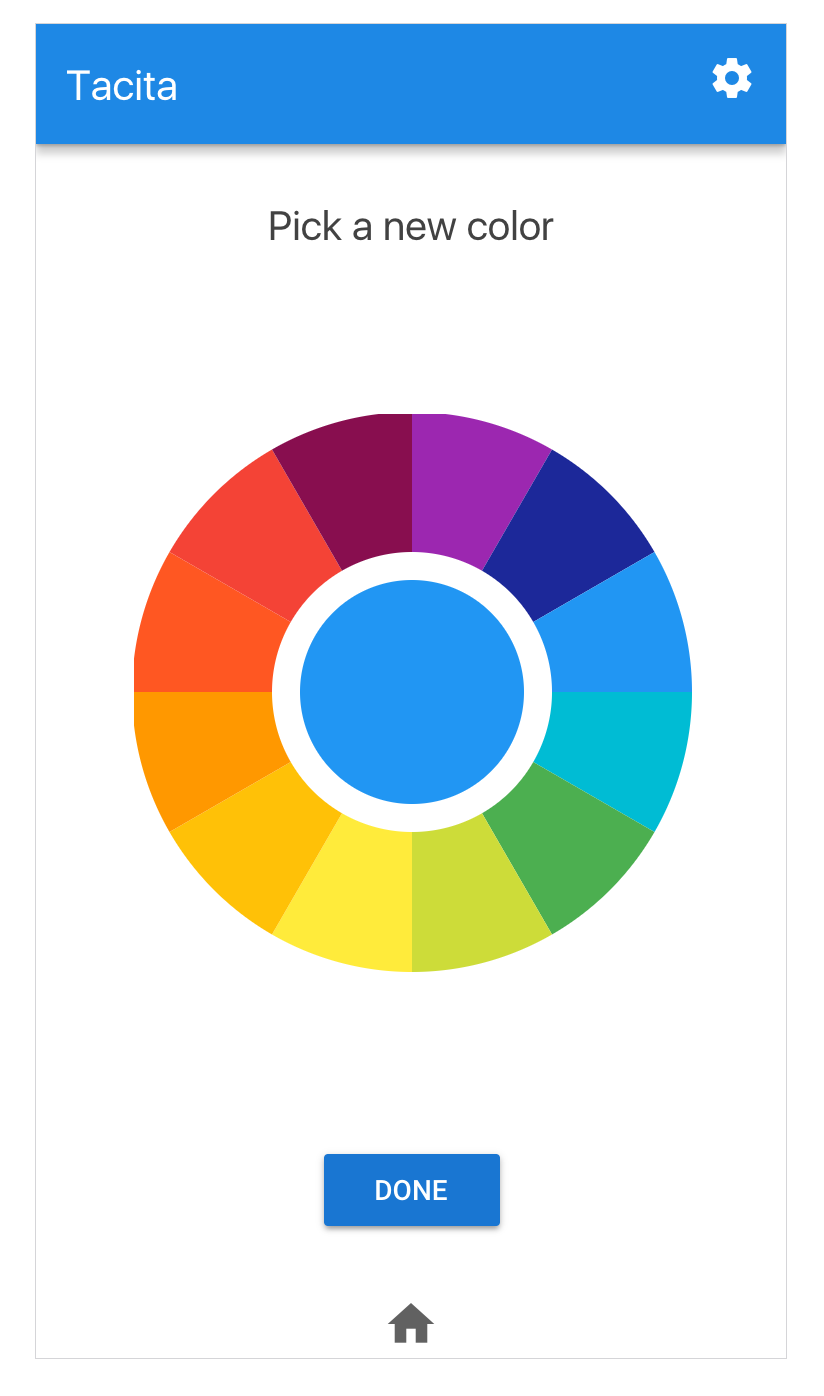
\includegraphics[width=0.25\textwidth]{./images/preference_colour/colour_select}}
   \
  \
  \
  \subfloat[Personalization page]{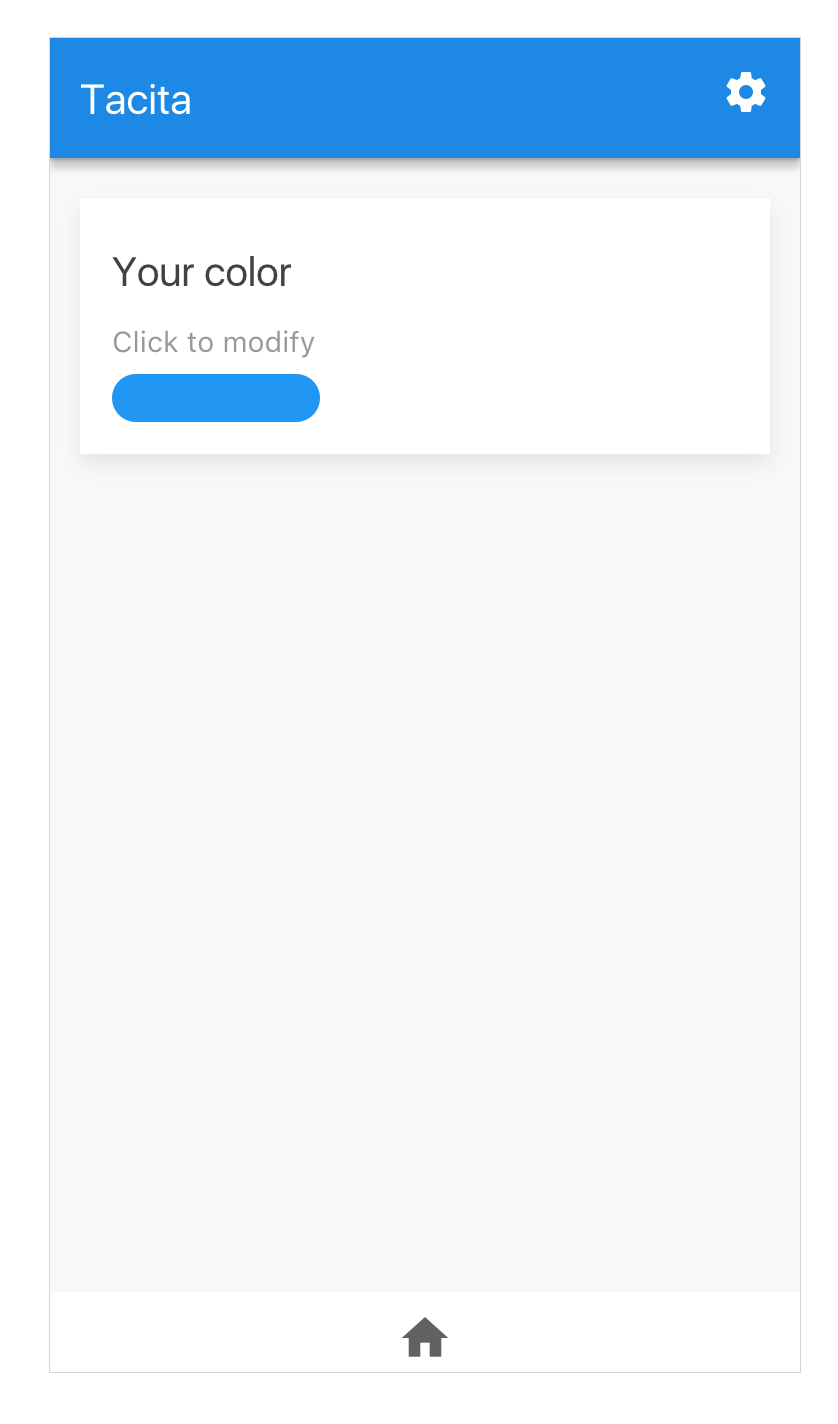
\includegraphics[width=0.25\textwidth]{./images/preference_colour/personalization_page}}
     \
  \
  \
    \subfloat[Appearence on a display]{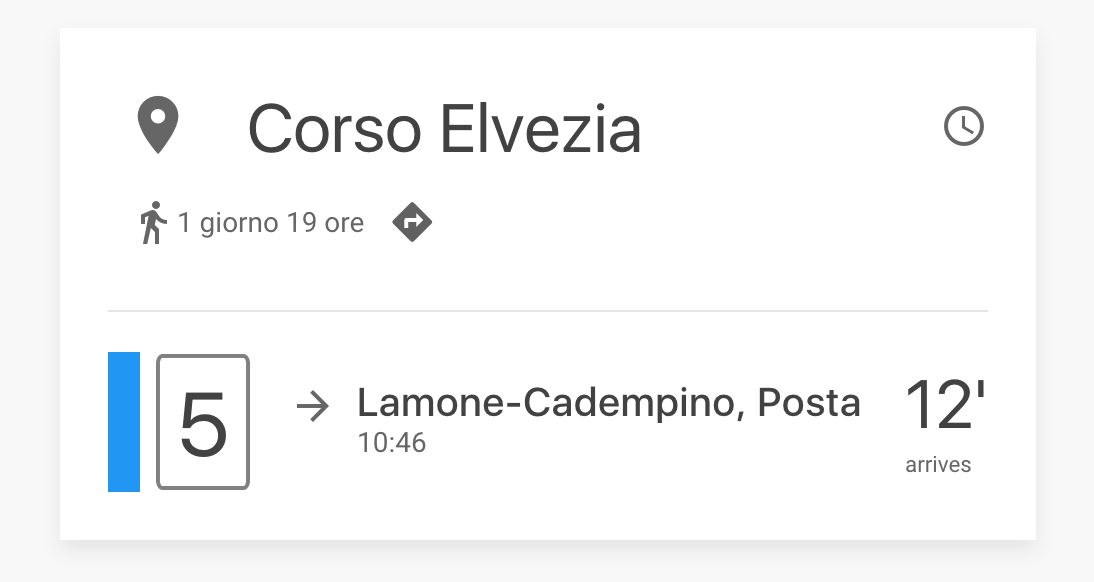
\includegraphics[width=0.25\textwidth]{./images/preference_colour/result}}
\end{figure}
In this example, the User selected a "blue" colour as identifier of his preferences. In figure \emph{u} you can see the actually final result on the display, a little labeled is added on the left part of the selected colour. If one of more users walk in, then the label is splitted.
\begin{figure}[H]
  \centering
  \subfloat[More users]{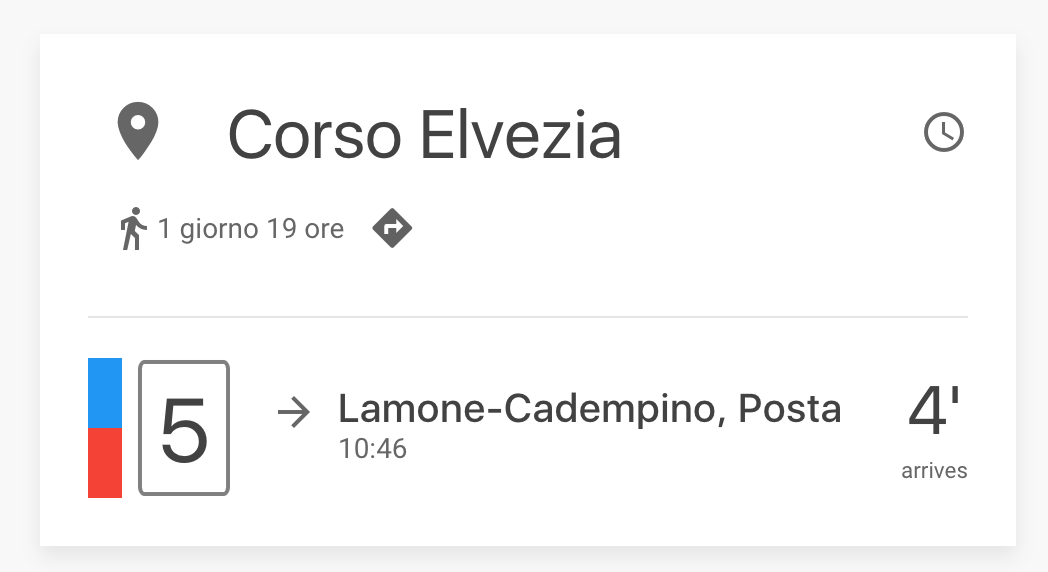
\includegraphics[width=0.25\textwidth]{./images/preference_colour/result_splitted}}
\end{figure}

\section{Conclusion}
Public displays are a powerful way to show content by interacting with it. With out system we showed that software can lead to improvement. The display, as it is, is a useless piece of hardware, but, combined with software it can becomes a better device. We started by exposing today's problem linked to a badly utilization of public screen showing, with examples, that they are mainly used for undirected advertisement.


After acknowledged such problems, we thought of a better system, in witch users are in control called \emph{Tacita}. In \emph{Tacita}, the displays becomes a real means of communication that can be dynamically adjust to target the correct user and the right time creating a new way of interaction. 

%%%%%
\newpage
\bibliographystyle{abbrv}
\bibliography{references}
\end{document}